\chapter{Power Measurement}
\label{sec:power_measurement}

\section{Validating RAPL Accuracy}
\label{sec:validating_rapl_accuracy}
Starting with the Sandy Bridge microarchitecture, Intel integrated current modelling into their processors to support power limiting~\cite{Hackenberg_2013_RAPL_APM}.
Haswell improved this by using current measurement~\cite{Hackenberg_2015_Haswell}.
The associated power metrics for different zones can be measured using the RAPL interface via the linux kernel~\cite{powercap_kernel_doc}.
Schöne et al.~\cite{Schoene_2024_Alder_Lake} tried to validate that RAPL counters on the Alder Lake architecture rely on current measurements.
However, they found that Intel is likely using a model for RAPL.
This is relevant to Sapphire Rapids, since they share the same core microarchitecture as Golden Cove.

\begin{figure}[]
    \centering
    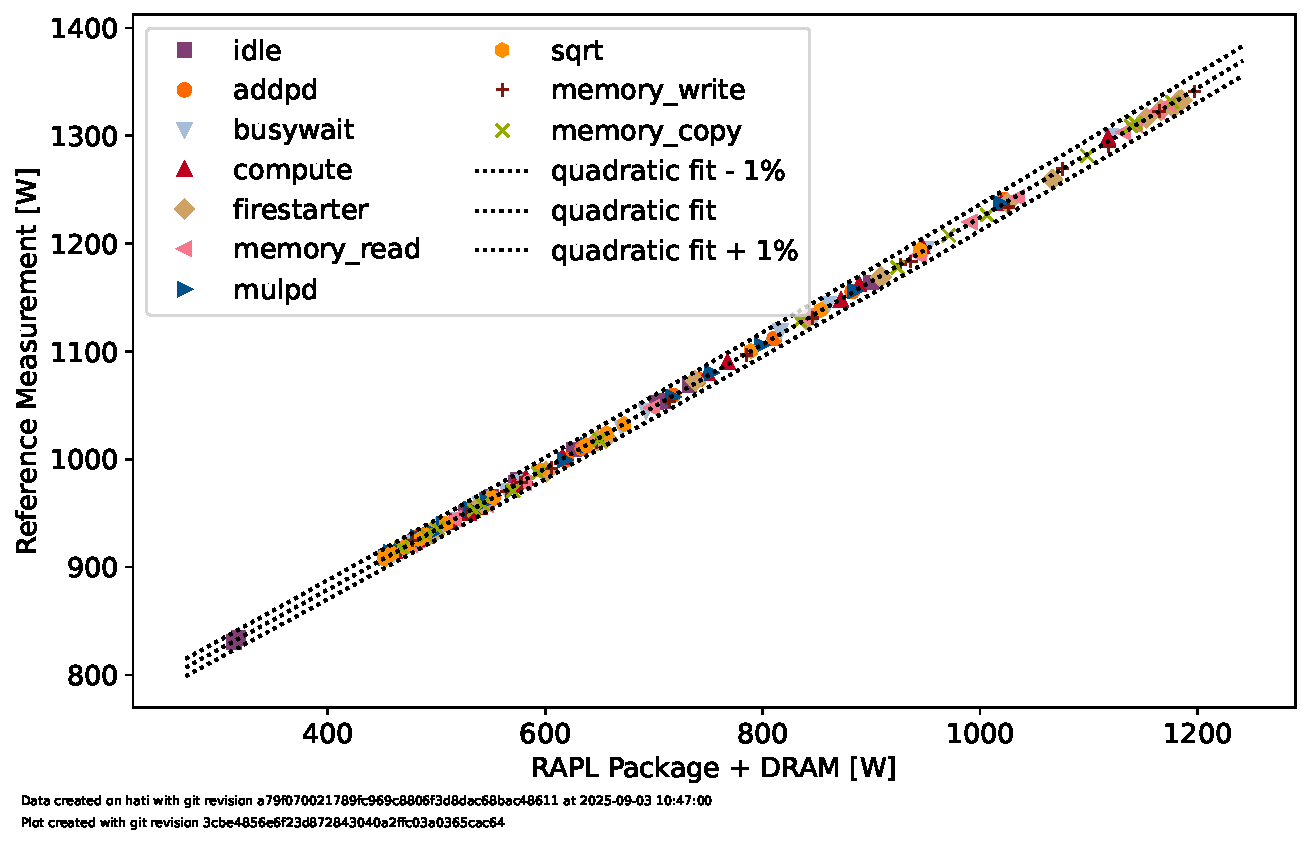
\includegraphics[width=0.8\columnwidth]{fig/rapl-accuracy/rapl-accuracy.pdf}
    \caption{\label{fig:validate-rapl}The roco2 microbenchmark is executed on a varying number of cores with different frequencies.
    The RAPL measurement can be mapped with a quadratic fit to the external reference measurement.}
\end{figure}

I validate the accuracy of these counters against an external measurement using the roco2 synthetic workload generator.
This software required some patches in order to to run on the current generation of processors.
They are documented in the forked GitHub repository~\footnote{\url{https://github.com/marenz2569/roco2/tree/marenz.hati-config}}.

Each of the displayed workload in~\figref{validate-rapl} were run for \SI{60}{\second} on the cross product of following settings:
\begin{itemize}
    \item Core frequency set to \SI{800}{\MHz}, \SI{1400}{\MHz}, \SI{2000}{\MHz} and \SI{3800}{\MHz} (turbo).
    \item Four settings which represent the execution of the workload on an increasing number of quadrants on the first socket.
    The number of cores used are: \SI{14}{}, \SI{28}{}, \SI{42}{} and \SI{56}{}.
\end{itemize}
The test matrix further included a full idle for each C-state setting (POLL, C1, C1E, C6).
Hyperthreading is disabled and the governor set to \texttt{performance}.
The power metrics are measured through the FIRESTARTER metric inferface.
This polls the RAPL metrics every \SI{10}{\ms} and discovered the first and last \SI{5}{\second} of each measurement duration.
The external reference measurent of the PDU is exposed via the metricq~\cite{Ilsche_2019_MetricQ} interface of FIRESTARTER~\footnote{\url{https://github.com/marenz2569/firestarter-metric-metricq}} and reports \SI{1}{Sa\per\second}.
The average power draw of the PDU and the RAPL counters are plotted in~\figref{validate-rapl}.
A strong correlation via quadratic fit can be observed, indicating that RAPL metrics use a measurement instead of a model.
The plots for the correlation of individual RAPL metrics are included in~\appref{validating_rapl_accuracy}.
All measurment points are inside the \SI{1}{\percent} tolerance of the PDU~\cite{Raritan_PX2_5528}.

\section{RAPL Filters}

Energy measurement with high accuracy can be used to measure the energy difference between different executed instructions and their data.
This has been demonstrated in great detail~\cite{Lucas_2016_AluPower,Schoene_2024_Alder_Lake,Schoene_2021_Zen2}.
However, it can also be used to perform side channel attacks and retrieve keys from priviledged programs~\cite{Lipp_2021_Platypus}.
While limiting access to the RAPL counters is possible from an operating system perspective, Intel also provides the option to enable filters \textbf{IA32\_MISC\_PACKAGE\_CTLS} on the energy measurement, which cannot be deactived until a reboot is performed~\cite[Vol. 4 Table 2-52]{intel_combined_software_developer_manual}.
The third generation of Xeon Scalable processors (Ice Lake) introduced the \textbf{MSR\_PACKAGE\_ENERGY\_TIME\_STATUS} MSR which also contains an accurate time point from when the measurement was performed.
This should address the problem of accurately measuring short code-paths as presented by Hähnel et al.~\cite{Haehnel_2012_RAPL}.

I extended the measurement for granularity of RAPL values proposed by Schöne et al.~\cite{Schoene_2024_Alder_Lake}.
All possible RAPL counters are polled repeatidly for \SI{10}{\s} on CPU 0 via their associated MSR.
CPU 1 runs FIRESTARTER to generate a constant power consumption on the processor.
The measurement is reapeated across the cross product of following settings:
\begin{itemize}
    \item All available core frequencies.
    \item With and without RAPL filters enabled.
    \item Both with all cstates and only POLL enabled.
    This causes two levels of power draw at the same frequency.
\end{itemize}
Only the counters \textbf{MSR\_PCKG\_ENERGY}, \textbf{MSR\_PACKAGE\_ENERGY\_TIME\_STATUS} and\\ \textbf{MSR\_RAM\_ENERGY} contain valid values.

I plot the package and DRAM counters for the nominal core frequency of \SI{2}{\GHz}.
\figref{rapl-update-intervals-package} shows the difference between the newly added timestamp in the model specific register\\ \textbf{MSR\_PACKAGE\_ENERGY\_TIME\_STATUS} and rdtsc as the source of the timestamp.
The package counter is updated every \SI{1.5}{\ms}.
It is increased to \SI{3.0}{\ms} with filters enabled.
\todoms{check that it is not 1.6}
The higher energy consumption when only enabling POLL is clearly visible.
Under the constant load scenario the timestamp of the RAPL register and the accumulated energy during this time follow a linear function, as is expected with accuracte timestamps.
Accurate timestamps seem to be deactived when the RAPL filter is enabled.
DRAM counters, displayed in \figref{rapl-update-intervals-dram} show an update interval of around \SI{1.6}{\ms}, this does not change with RAPL filters enabled.
DRAM counters are not as accurate as the package counters, but also do not show such a big spread when using rdtsc as the timestamp source.

Data center and HPC administrators require accuracte energy accounting of larger code paths or accross multiple executions, software developers require it for fast runtime optimization of energy efficiency.
An increased accuracy of this measurement is possible with the use of the internal timestamp in the \textbf{MSR\_PACKAGE\_ENERGY\_TIME\_STATUS} register.
For use cases with security critical data and algorithms, I recommend to activate the filter thus increasing the barrier against leaks, even if parts of the system are compromised.

\begin{figure}[]
    \centering
    % width could be 1, 0.9, 0.8 instead
    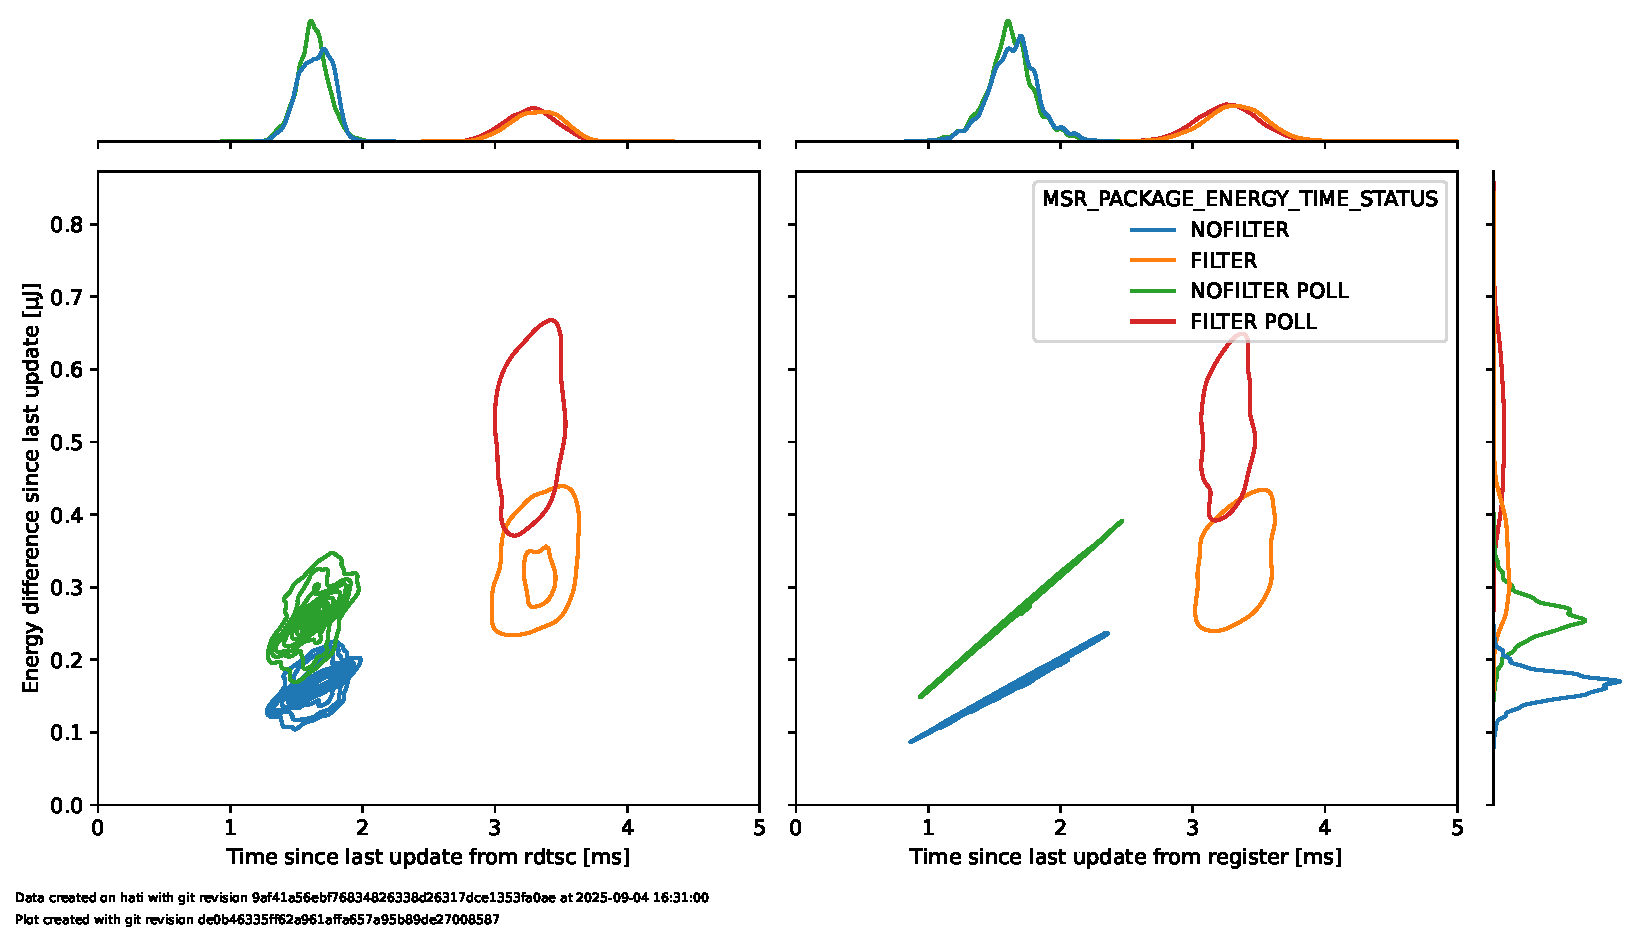
\includegraphics[width=\columnwidth]{fig/rapl-update-intervals/MSR_PACKAGE_ENERGY_TIME_STATUS_2000000.pdf}
    \caption{\label{fig:rapl-update-intervals-package}Kernel density estimation of the time of measurement vs read energy value of the RAPL package counter of the first socket during for two constant power draw scenarios with and without filters enabled.
    The left plot uses the \textbf{rdtsc} function to get a timestamp for the RAPL measurement, the right uses the newly integrated timestamp in the \textbf{MSR\_PACKAGE\_ENERGY\_TIME\_STATUS} MSR.}
\end{figure}

\begin{figure}[]
    \centering
    % width cloud be 0.54, 0.49, 0.44 instead
    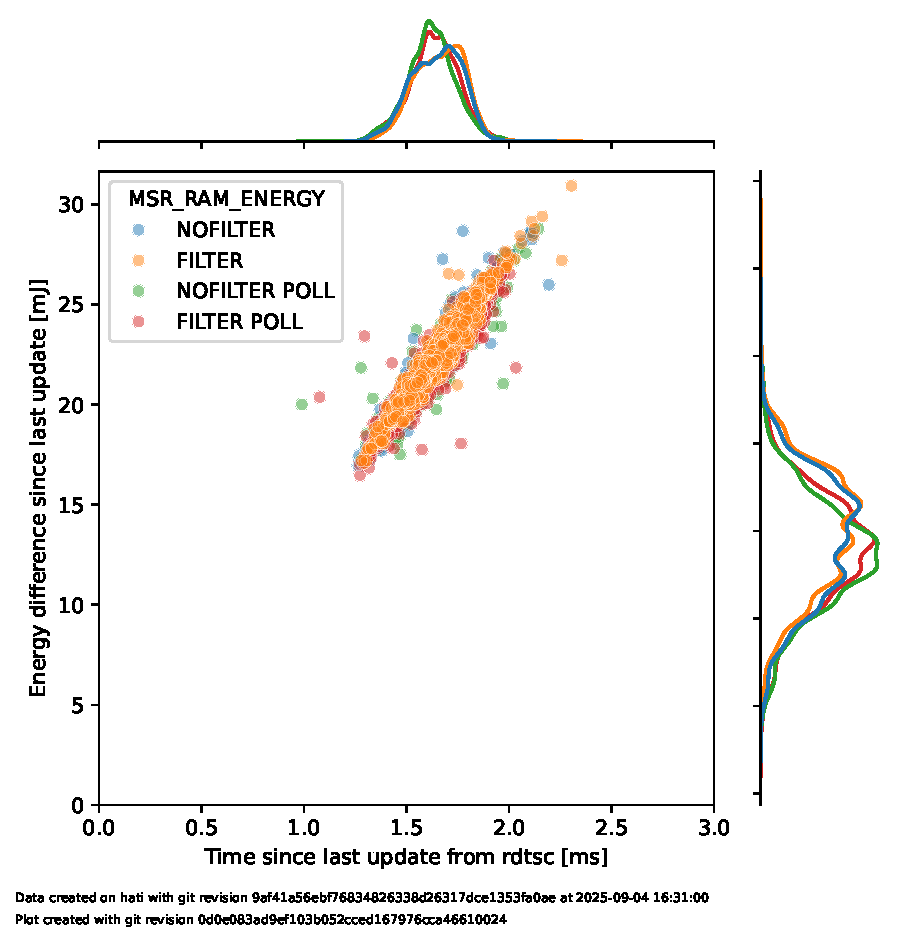
\includegraphics[width=0.54\columnwidth]{fig/rapl-update-intervals/MSR_RAM_ENERGY_2000000.pdf}
    \caption{\label{fig:rapl-update-intervals-dram}Kernel density estimation of the time of measurement via timestamp counter and the read energy value of the RAPL dram counter of the first socket during a constant power draw scenario.}
\end{figure}